%\chapter{Introduction to Linear Programming}
\chapter{Connectivity}
\section{Bipartite Graphs}
\begin{definition}[Cycle]
A \emph{cycle} is a sequence of adjacent edges
\[
\begin{array}{lllll}
(v_0,v_1),
&
(v_1,v_2),
&
\dots,
&
(v_{m-2},v_{m-1}),
&
(v_{m-1},v_m=v_0)
\end{array}
\]
where all the vertices $v_0,v_1,\dots,v_{m-1}$ are \emph{distinct}.
The number of deges in the cycle is called its \emph{length}.
\end{definition}

\begin{definition}[Bipartite]
A graph $G=(V,E)$ is \emph{bipartite} if its vertex-set is a union of two disjoint sets, say $A$ and $B$,
such that every edge in $E$ joins a vertex in $A$ to one in $B$.
\end{definition}

\begin{theorem}
A graph $G$ is \emph{bipartite} if and only if every cycle of $G$ has even length.
\end{theorem}
\begin{proof}
\textit{Necessity}.
Take any cycle and ``trace'' its edges, the cylce must have even length.

\textit{Sufficiency}.
w.l.o.g., $G$ is connected.
Construct $A$ as the vertices s.t. the shortest path to $v$ has even length. Then $B$ is the set of vertices that are not in $A$.

We claim that $(A,B)$ forms a bipartite graph, since otherwise we can construct a cycle with odd length.
\end{proof}

\section{Bounds on the number of edges}

\begin{definition}[Connected]
A graph is \emph{connected} if there is a path from every vertex to any other vertex
\end{definition}
\begin{definition}[Simple]
A graph is \emph{simple} if there are no parallel edges nor loops.
\end{definition}
The goal is to give a bound on a simple connected graph with $n$ vertices.

\begin{definition}[Connected]
\begin{enumerate}
\item
If $G_1=(V_1,E_1)$ and $G_2=(V_2,E_2)$ are graphs,
and the vertex sets $V_1$ and $V_2$ are disjoint,
then their \emph{union} is the graph $G=(V_1\cup V_2,E_1\cup E_2)$
\item
A graph is \emph{connected} if it cannot be expressed as a union of graphs, and disconnected otherwise.
\end{enumerate}
\end{definition}

\begin{definition}[Component]
Any \emph{disconnected} graph $G$ can be expressed as a union of connected graphs, each of which is called a \emph{component} of $G$.
\end{definition}

\begin{theorem}\label{The:2:2}
Let $G$ be a simple graph on $n$ vertices with $k$ componets.
The number $m$ of edges of $G$ satisfies
\[
n-k\le m\le (n-k)(n-k+1)/2.
\]
\end{theorem}
\textit{Lower Bound (By induction on the number of edges):}
The lower bound is true for a null graph $G$.
We assume the lower bound holds true for number of edges less than $m_0$.
Consider a graph $G$ (suppose that it has $n$ vertices and $k$ components) with \emph{minimal} edges, say $m_0$, i.e., removing one edge will increase the number of components by $1$. Therefore, the resultant graph has $n$ vertices, $k+1$ components and $m_0-1$ edges. By the induction hypothesis, we imply
\[
n-(k+1)\le m_0-1\implies
n-k\le m_0.
\]

\textit{Upper bound:}
It suffices to consider the case where each component of $G$ is a complete graph (since we are considering the upper bound).
Suppose that there are two components $C_i$ and $C_j$ with $n_i$ and $n_j$ vertices, respectively, and $n_i\ge n_j>1$.

Now we argue that $n_i$ should be larger than $n_j$ as much as possible ($n_i+n_j$ keeps the same) to obtain more vertices:
Consider the components $B_i$ and $B_j$ with $n_i+1$ and $n_j-1$ vertices, respectively.
Then the toal number of vertices remains unchanged, but the total number of edges is more than the previous one:
\[
\frac{n_i(n_i+1)}{2}+\frac{(n_j-2)(n_j-1)}{2}
-
\frac{(n_i-1)n_i}{2}-\frac{n_j(n_j-1)}{2}
=
n_i-n_j+1>0.
\]
Therefore, in order to obtain the maximum number of edges, $G$ must consists of a complete graph with $n-k+1$ vertices and $k-1$ isolated vertices.

\begin{corollary}
If a simple graph on $n$ vertices has more than $(n-1)(n-2)/2$ edges, it must be connected.
\end{corollary}
\begin{proof}
The key insight is that the graph with more componets should have less vertices. The vertices for the graph with more than 1 components is upper bounded by $(n-1)(n-2)/2$, by applying Theorem~(\ref{The:2:2}).
\end{proof}
\section{Edge $\&$ Vertex Connectivity}
\begin{definition}[Disconneting Set]
A \emph{disconnecting (edge) set} of a graph $G$ is a set of edges whose removal increases the number of components of $G$
\end{definition}
\begin{definition}[Cutset]
A \emph{cutset} of a graph $G$ is a \emph{minimal disconnecting set};
a cut-set of size 1 is called a \emph{bridge}
\end{definition}
\begin{definition}[Edge-Connectivity]
For connected graph $G$, its \emph{edge-connectivity} $\lambda(G)$ is the number of edges of the smallest cutset of $G$. 
In other words, $\lambda(G)$ is the fewest number of edges to be removed such that the resulting graph is dis-connected.

We say $G$ is \emph{$k$-edge connected} if $\lambda(G)\ge k$
\end{definition}
\begin{definition}[Separating Vertex Set]
A \emph{separating vertex set} of a connected graph $G$ is a set of vertices whose deletion (together with their incident edges) disconnects $G$;
we say $v$ is a \emph{cut-vertex} if a separating set has only one vertex $v$.
\end{definition}

\begin{definition}[Vertex-Connectivity]
For connected graph $G$, its \emph{vertex-connectivity} $\kappa(G)$ is the minimum size $S$ such that $G-S$ is disconnected or has only one vertex.

We say $G$ is \emph{$k$ (-vertex) connected} if $\kappa(G)\ge k$.
\end{definition}
For example, $\kappa(K_n) = n-1$, where $K_n$ denotes a complete graph with $n$ vertices.

The Theorem~(\ref{The:2:4}) shows that the vertex-connectivity is more intrinsical than the edge-connectivity.
\begin{theorem}\label{The:2:4}
For a connected graph $G$, we have
\[
\kappa(G)\le\lambda(G)\le\delta(G),
\]
where $\delta(G)$ denotes the smallest vertex-degree of $G$.
\end{theorem}
\begin{proof}
\textit{Upper Bound}:
The upper bound is trivial, since removing all the edges of the vertex with smallest degree will lead to a disconnected graph, i.e., $\lambda(G)\le\delta(G)$.

\textit{Lower Bound}: Skipped, since not understand.
\end{proof}

\begin{example}
It's possible for both inequality in Theorem~(\ref{The:2:4}) to be strict:
\begin{figure}[H]
\centering
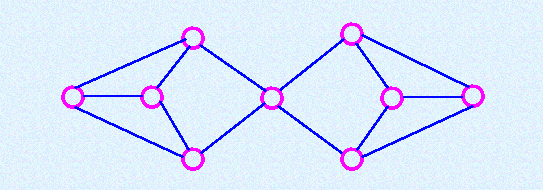
\includegraphics[width=0.7\textwidth]{Second_lecture/p_10}
\end{figure}
In such case, $\kappa(G)=1,\lambda(G) = 2,\delta(G)=3$.
\end{example}

\begin{theorem}[Menger's Theorem]
A graph $G$ is \emph{$k$-edge-connected} if and only if any two distinct vertices of $G$ are joined  by at least $k$ disjoint paths, i.e., no two of which have any edge in common.
\end{theorem}
\begin{theorem}[Menger's Theorem]
A graph with at least $k+1$ vertices is $k$-connected if and only if any two distinct vertices of $G$ are joined by at least $k$ disjoint paths.
\end{theorem}

\begin{definition}[Disconnecting Set]
A $vw$-disconnecting set of a graph $G$ is a set of edges $F$ of $G$ such that
every path from $v$ to $w$ includes an edge of $F$.
\end{definition}
\begin{theorem}[Menger's Theorem (edge form)]
The \emph{maximum number of edge-disjoint paths} connecting two distinct vertices $v$ and $w$ of a connected graph is equal to the \emph{minimum number of edges in a $vw$-disconnecting set}.
\end{theorem}
\begin{proof}
It's trivial that the the maximum number of edge-disjoint paths cannot be more than the number of edges in a $vw$-disconnecting set.

The reverse direction relies on the induction on the number of edges.
\end{proof}
\paragraph{From Eulerian Problem into the Chinese Postman Problem}
Recall that a connected graph is \emph{Eulerian} if there exists a closed trail that includes every edge of $G$. The necessary and sufficient condition is that every vertex has even degree.

When a graph is not Euliean, we want to find a walk that covers all the edges, but avoid repeating  edges as much as possible. Or equivalently, how many and which edges need to be duplicated such that the resultant is Eulerian? This motivates the Chinese Postman Problem.

\begin{definition}[The Chinese Postman Problem]
A postman has to deliver letters to a given neighbourhood. He needs to walk through all the streets in the neighbourhood and back to the post office. How can he design his route so that he walks the shortest distance?
\end{definition}

\begin{definition}[Connected]
A directed graph $G$ is connected if the corresponding underlying graph is connected
\end{definition}
\begin{definition}[Strongly Connected]
A directed graph $G$ is \emph{strongly connected} if for any vertex $v$ and $w$, there is a directed path from $v$ to $w$
\end{definition}
\begin{definition}[Orientable]
We say an \emph{undirected} graph is \emph{orientable} if each edge can be \emph{directed} such that the resulting graph is \emph{strongly connected}.
\end{definition}

\begin{theorem}
A connected graph is \emph{orientable} if and only if every edge of $G$ lies in at least one cycle.
\end{theorem}

\begin{proof}[Sufficiency]
Choose any cycle $C$ and direct its edges \emph{cyclically}.
If all edges of $G$ have been oriented, the proof is complete; otherwise choose an edge, say $e$, that is not in $C$ but adjacent to an edge of $C$.
By hypothesis, the edge $e$ is in some cycle $C'$, and orient the edges in $C'$ cyclically except for those already directed.

We proceed this operation, and thus directing at least one more edge for each time.
Therefore, we are done until all edges have been oriented.
The oriented edges form a strongly-connected graph.
\end{proof}


















